\chapter{Heap Binomiali}
Gli heap binomiali fanno parte di una famiglia di Heap detta mergeable Heap che consistono in degli heap che supportano, oltre che le classiche operazioni, anche l'unione tra due heap.
\section{Alberi binomiali}
Prima di parlare di heap binomiali, è necessario parlare di alberi binomiali che sono la compenente fondamentale utilizzata negli heap binomiali.
Per ogni $k\in N$ esiste un albero binomiale $B_k$ di grado k definito in basse alla seguente ricorsione:
\begin{itemize}
    \item $B_0$ è l'albero formato da un solo nodo.
    \item Dato $B_{k-1}$ definiamo $B_k$ come la combinazione di due alberi di grado $k-1$ per cui la radice più grande \footnote{O più piccola nel caso di un max heap} và alla sinistra della radice più piccola. Sulla base di questa proprietà, possiamo dire che gli alberi binomiali così definiti sono \textbf{ordinati.}
    \begin{figure}[H]
        \centering
        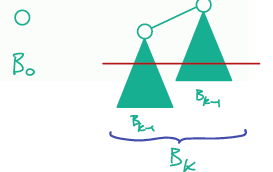
\includegraphics[width=0.5\linewidth]{Images/capitolo_heap_binomiale/combinazione_albero_binom.png}
    \end{figure}
\end{itemize}
Gli alberi binomiali seguono alcune particolar proprietà importanti da avere in mente:
\begin{enumerate}
    \item L'albero $B_k$ di grado $k$ ha esattamente $2^k$ nodi.
    \item L'altezza di $B_k$ è K.\footnote{Cammino più lungo dalla radiche ad una foglia.}
    \item $B_k$ ha $\binom{k}{i}$ nodi a profondità i.
    \item La radice di $B_k$ ha grado k ed ogni altro nodo in $B_k$ ha grado inferiore a k. Inoltre i figli di $B_k$ sono radici di $B_{k-1},B_{k-2},\dots,B_0$ in questo esatto ordine.
    \begin{figure}[H]
        \centering
        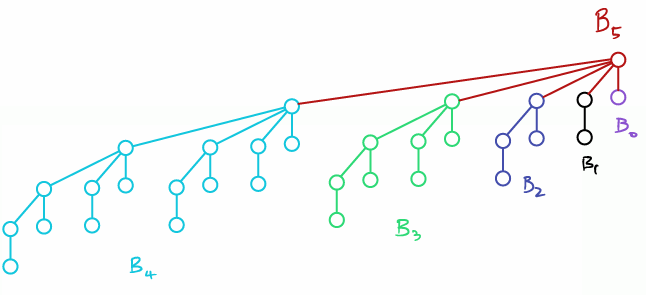
\includegraphics[width=0.5\linewidth]{Images/capitolo_heap_binomiale/albero_binom_ordine.png}
    \end{figure}
\end{enumerate}
Queste proprietà possono essere dimostrate tramite induzione.\\
\textbf{DIMOSTRAZIONE}\\
Caso base:
\begin{itemize}
    \item $B_0$ ha 1 nodo che equivale a $2^0$.
    \item L'altezza di $B_0$ è 0.
    \item $B_0$ ha $\binom{0}{0}=1$ nodi a profondità 0.
    \item La radice di $B_0$ ha grado 0.
\end{itemize}
Passo induttivo:
\begin{enumerate}
    \item $B_k$ ha $\#(B_k)=\#(B_{k-1})+\#(B_{k-1}) = 2^{k-1}+2^{k-1}= 2^k$.
    \item L'altezza di $B_k$ è uguale a $h(B_{k-1})+1=(k-1)+1=k$.
    \item Considerando un albero $B_k$, questo è composto dagli alberi $B_{k-1}', B_{k-1}''$. Supponiamo che $B_{k-1}'$ sia l'albero a cui attacca la radice di $B_{k-1}''$. Noteremo che, per quanto riguarda i nodi al livello d dell'albero $B_{k-1}'$, questi non saranno cambiati poiché l'albero è rimasto fermo. La situazione è diversa per l'albero $B_{k-1}''$ i cui livelli sono scesi di uno. Da qui, avremo che:
    \[Nodi_d = \binom{k-1}{d}+\binom{k-1}{d-1} = \binom{k}{d}\]
    \item Il grado della radice di $B_k$ è $deg(B_{k-1}+1)=k-1+1=k$. Ciascun nodo di $B_{k-1}$ ha, per ipotesi induttiva, un grado inferiore a k-1 per cui anche inferiore a k. Il primo figlio della radice di $B_k$ è radice di $B_{k-1}$ per cui è già in ordine. Di conseguenza, per ipotesi induttiva, i successivi $k-1$ figli sono radici di $B_{k-2},\dots,B_1$. 
\end{enumerate}
\textbf{COROLLARIO}\\
Sia B un albero binomiale con n nodi, allora ogni nodo in B ha grado al più $log(n)$.\\
\textbf{DIMOSTRAZIONE}\\
Per qualche $k\in N $ avremo $B=B_k$, quindi $n=2^k.$ Ogni nodo ha grado $\leq k$ ma $k=log(n)$ da qui la tesi.

\section{Heap binomiali}
Uno Heap Binomiale $H$ non è altro che una foresta di alberi binomiali ordinati per grado crescente tali che:
\begin{itemize}
    \item Ogni albero in $H$ gode della proprietà di min-heap.
    \item Per ogni $k\in N$, H contiene solo un albero di grado k.
\end{itemize}
Da qui naturalmente notiamo come, per ogni albero, la radice sia la chiave minima e, per ogni heap con n nodi, ci sono al più $\lfloor log(n) \rfloor + 1$ alberi binomiali. Ogni nodo è composto dalla chiave, dal suo grado, dal padre, dai fratelli e da un puntatore ad un solo figlio.\footnote{Nel caso volessimo trovare tutti gli altri figli, ci basterebbe ispezionare tutta la lista di fratelli del figlio}
\begin{figure}
    \centering
    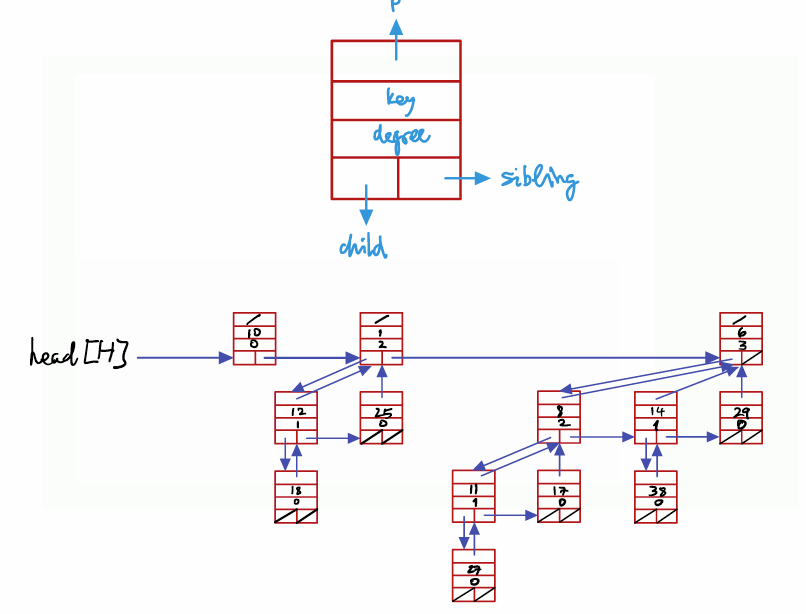
\includegraphics[width=0.5\linewidth]{Images/capitolo_heap_binomiale/esempio_heap_binomial.png}
\end{figure}
\section{Operazioni Heap Binomiali}
Tra le varie operazioni basilari troviamo:
\begin{itemize}
    \item Make-Binomial-Heap().
    \item Binomial-Heap-Minimum(H).
    \item Binomial-Link(y,z).
    \item Binomial-Heap-Union($H_1,H_2$). 
    \item Binomial-Heap-Insert($H,x$).
    \item Binomial-Heap-Extract-min($H$).
    \item Binomial-Heap-Decrease-key($H,x,k$).
    \item Binomial-Heap-Delete(x).
\end{itemize}

\subsection{Make-Binomial-Heap()}
Questa operazione permette la creazione di un heap binomiale vuoto.
\begin{algorithm}[H]
\caption{MAKE-BINOMIAL-HEAP()}
\begin{algorithmic}[1]
    \State $H \gets \textsc{Allocate-Heap}()$
    \State $head[H] \gets \textbf{NIL}$
    \State \Return $H$
\end{algorithmic}
\end{algorithm}
La complessità di questo algoritmo sarà $O(1)$.
\subsection{Binomial-Heap-Minimum(H)}
Questa operazione permette di trovare il minimo nello heap. 
\begin{algorithm}[H]
\caption{BINOMIAL-HEAP-MINIMUM($H$)}
\begin{algorithmic}[1]
    \State $y \gets \textbf{NIL}$
    \State $x \gets head[H]$
    \State $min \gets \infty$
    \While{$x \neq \textbf{NIL}$}
        \If{$key[x] < min$}
            \State $min \gets key[x]$
            \State $y \gets x$
        \EndIf
        \State $x \gets sibling[x]$
    \EndWhile
    \State \Return $y$
\end{algorithmic}
\end{algorithm}
La complessità di questo algoritmo è $O(log(n))$ poiché, come detto prima, è possibile che vi siano al più $log(n)$ alberi binomiali.

\subsection{Binomial-Link(y,z)}
 Grazie a questa operazione possiamo unire due alberi y,z dello stesso grado per dare vita ad un albero di grado maggiore.
\begin{algorithm}[H]
\caption{BINOMIAL-LINK($y, z$)}
\begin{algorithmic}[1]
    \State $p[y] \gets z$
    \State $sibling[y] \gets child[z]$
    \State $child[z] \gets y$
    \State $degree[z] \gets degree[z] + 1$
\end{algorithmic}
\end{algorithm}
\begin{figure}[H]
    \centering
    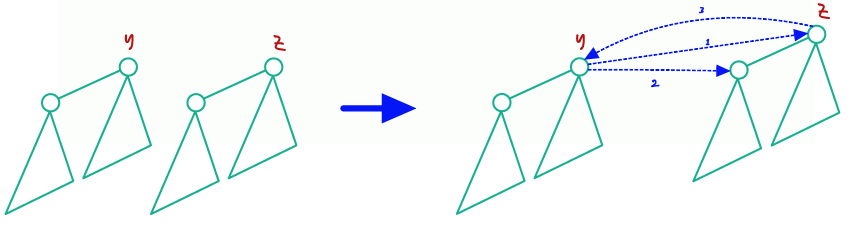
\includegraphics[width=0.5\linewidth]{Images/capitolo_heap_binomiale/link_tra_alberi.png}
\end{figure}

\subsection{Binomial-Heap-Union($H_1,H_2$)}
Questa operazione è la chiave di tutto lo Heap. In pratica permette di unire due heap binomiali rispettando tutte le proprietà sopra citate. L'idea alla base di questa procedura è quella di eseguirla come se fosse una somma tra due numeri binari, eseguendola in questo modo.
\begin{figure}[H]
    \centering
    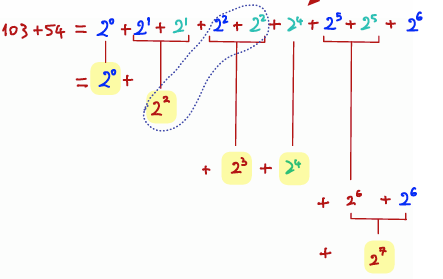
\includegraphics[width=0.5\linewidth]{Images/capitolo_heap_binomiale/esempio_somma_binari.png}
\end{figure}
Come possiamo vedere, non facciamo altro che mettere in ordine il tutto e cominciamo ad eseguire le somme di volta in volta e, quando incontriamo tre numeri uguali,\footnote{Che nel caso degli alberi saranno le radici con lo stesso grado} ne ignoriamo uno e facciamo la somma solo tra gli altri due. Vediamo al procedura:
\begin{algorithm}[H]
\caption{BINOMIAL-HEAP-UNION($H_1, H_2$)}
\begin{algorithmic}[1]
    \State $H \gets \textsc{Make-Binomial-Heap}()$ \Comment{Creazione di un nuovo albero}
    \State $head[H] \gets \textsc{Binomial-Heap-Merge}(H_1, H_2)$ \Comment{Si uniscono i due heap nello heap appena creato mettendo in ordine di grado gli alberi}
    \State \textit{free the objects $H_1$ and $H_2$ but not the lists they point to}
    \If{$head[H] = \textbf{NIL}$}
        \State \Return $H$
    \EndIf
    \State $prev\text{-}x \gets \textbf{NIL}$
    \State $x \gets head[H]$
    \State $next\text{-}x \gets sibling[x]$
    \While{$next\text{-}x \neq \textbf{NIL}$} \Comment{Scorriamo la lista}
        \If{$(degree[x] \neq degree[next\text{-}x])$ \textbf{or} $(sibling[next\text{-}x] \neq \textbf{NIL}$ \textbf{and} $degree[sibling[next\text{-}x]] = degree[x])$} \Comment{Se abbiamo due gradi diversi tra il primo e il secondo o sia il primo che il terzo hanno lo stesso grado, scorriamo}
            \State $prev\text{-}x \gets x$
            \State $x \gets next\text{-}x$
        \ElsIf{$key[x] \leq key[next\text{-}x]$} \Comment{Se hanno lo stesso grado e il primo è più piccolo del secondo, il secondo si attacca al primo.}
            \State $sibling[x] \gets sibling[next\text{-}x]$
            \State \textsc{Binomial-Link}$(next\text{-}x, x)$
        \Else \Comment{Caso speculare a quello prima ma il primo si attacca al secondo}
            \If{$prev\text{-}x = \textbf{NIL}$}
                \State $head[H] \gets next\text{-}x$ \Comment{Se necessario, aggiorniamo la testa}
            \Else
                \State $sibling[prev\text{-}x] \gets next\text{-}x$
            \EndIf
            \State \textsc{Binomial-Link}$(x, next\text{-}x)$
            \State $x \gets next\text{-}x$
        \EndIf
        \State $next\text{-}x \gets sibling[x]$
    \EndWhile
    \State \Return $H$
\end{algorithmic}
\end{algorithm}
Analizziamo la complessità di questo algoritmo. Chiamiamo $n_1, n_2$ il numero di nodi dei rispettivi alberi. Sappiamo che \[n\geq n_1+n_2\leq \lfloor log(n_1) \rfloor + \lfloor log(n_2) \rfloor+2\leq 2 \lfloor 2log(n) \rfloor+2\] Per cui, la complessità del merge è $O(log(n))$. Ogni iterazione del ciclo, x o và avanti di una posizione o viene fatto un link che ha tempo 
costante. Per tanto, questo algoritmo ha complessità $O(log(n)).$

\subsection{Binomial-Heap-Insert($H,x$)}
Tramite questa operazione, facciamo un'inserimento nello heap che non è altro che la crazione di un heap con un solo nodo con cui poi si fa' l'unione.
\begin{algorithm}[H]
\caption{BINOMIAL-HEAP-INSERT($H$, $x$)}
\begin{algorithmic}[1]
    \State $H' \gets \textsc{Make-Binomial-Heap}()$
    \State $p[x] \gets \textbf{NIL}$
    \State $child[x] \gets \textbf{NIL}$
    \State $sibling[x] \gets \textbf{NIL}$
    \State $degree[x] \gets 0$
    \State $head[H'] \gets x$
    \State $H \gets \textsc{Binomial-Heap-Union}(H, H')$
\end{algorithmic}
\end{algorithm}
La complessità sarà $O(log(n))$ poiché dipenderà tutto dalla union.

\subsection{Binomial-Heap-Extract-min($H$)}
Questa operazione consiste nell'eliminazione del minimo.
\begin{algorithm}[H]
\caption{BINOMIAL-HEAP-EXTRACT-MIN($H$)}
\begin{algorithmic}[1]
    \State \textit{Troviamo la radice $x$ con chiave minima e la rimuoviamo stacchiamo dalla lista.}
    \State $H' \gets \textsc{Make-Binomial-Heap}()$
    \State \textit{Eliminiamo la radice x dalla parte che abbiamo staccato e facciamo puntare la testa del nuovo heap alla lista dei figli di x però invertita. Invertendola avremo di nuovo l'ordine crescente}
    \State $H \gets \textsc{Binomial-Heap-Union}(H, H')$ \Comment{Riuniamo il tutto tramite la union}
    \State \Return $x$
\end{algorithmic}
\end{algorithm}
Anche in questo caso avremo che la complessità sarà $O(log(n))$.

\subsection{Binomial-Heap-Decrease-key($H,x,k$)}
Questa operazione permette di portare la chiave del nodo x ad un valore k inferiore al valore della chiave precedente. In questo caso supporremo già di avere un puntatore che punta al nodo x.

\begin{algorithm}[H]
\caption{BINOMIAL-HEAP-DECREASE-KEY($H, x, k$)}
\begin{algorithmic}[1]
    \If{$k > key[x]$}
        \State \textbf{error} "new key is greater than current key"
    \EndIf
    \State $key[x] \gets k$
    \State $y \gets x$
    \State $z \gets p[y]$
    \While{$z \neq \textbf{NIL}$ \textbf{and} $key[y] < key[z]$}
        \State \text{exchange } $key[y] \leftrightarrow key[z]$
        \Statex{If y and z have satellite fields, exchange them, too.}
        \State $y \gets z$
        \State $z \gets p[y]$
    \EndWhile
\end{algorithmic}
\end{algorithm}

In questo caso la complessità sarà anche qui $O(log(n))$ poiché non facciamo altro che scambiare le chiavi fino a far salire quella cambiata al punto giusto dell'albero che avrà al massimo $log(n)$ livelli.

\subsection{Binomial-Heap-Delete(x)}
Tramite l'operazione di delete non facciamo altro che andare ad eliminare uno specifico nodo x. E, grazie alle operazioni che abbiamo definito prima, questa è un'operazione ormai banale. 

\begin{algorithm}[H]
\caption{BINOMIAL-HEAP-DELETE($H, x$)}
\begin{algorithmic}[1]
    \State \textsc{Binomial-Heap-Decrease-Key}($H, x, -\infty$)
    \State \textsc{Binomial-Heap-Extract-Min}($H$)
\end{algorithmic}
\end{algorithm}

La complessità sarà anche qui $O(log(n))$.
\section{Analisi ammortizzata di un inserimento in uno heap binomiale inizialmente vuoto}
Scegliamo come funzione potenziale $\Phi(H)$ il numero di alberi binomiali in uno heap. Per cui, se $H_0$ è un albero binomiale vuoto, avremo che $\Phi(H)\geq \Phi(H_0)$. Il costo reale $c_i$ è dato da:
\[c_i=\#\text{Make-binomial-heap}+\#\text{binomial-link}\]
Il costo ammortizzato di una make-binomial-heap è:
\[c_i'=c_i+\Delta\Phi=1+0=1\]
Dunque, il costo di un inserimento è 
\begin{align*}
    &c_i'=c_i+\Delta\Phi\\
    &=(1+\#Link_i)+(\#alberi_i-\#alberi_{i-1})=\\
    &=(1+\#Link_i)+((\#alberi_{i-1}+1-\#Link_i)-\#alberi_{i-1}) = 2
\end{align*}
Quindi n inserimenti in un heap binomiale inizialmente vuoto possono essere effettuati in tempo $O(n)$.

\chapter{Heap di Fibonacci}
Uno Heap di Fibonacci è anch'esso una collezione di alberi binomiale che, però, non sono ordinati ma mantengono comunque la proprietà di min heap.
In un certo senso, possiamo dire che questi somiglino agli Heap binomiali con alcune differenze sostanziali:
\begin{enumerate}
    \item Se negli heap binomiali abbiamo una lista ordinata, qui abbiamo una \textbf{lista non ordinata} e che è \textbf{circolare}.
    \item Negli heap di Fibonacci è ammesso avere più alberi dello stesso grado. 
    \item Gli alberi in questo caso, pur seguendo una certa logica, non risultano essere ordinati e non sono binomiali.
\end{enumerate}
 Un'altra cosa da sottolineare è che questi alberi possono essere "degradati" attraverso alcune procedure di cui parleremo in seguito che, però, proprio grazie alla degradazione, avranno tempi ammortizzati costanti. Dimostreremo, infatti, che Extract min e Delete hanno complessità O(D(n)) dove D(n) rappresenta il massimo grado di un nodo nell’heap che sarà $\leq n-1$ e, \footnote{Ciò accade perché la peggiore situazione possibile, avendo n nodi, è che ad un solo nodo colleghiamo tutti gli altri e, questo, avrebbe quindi grado n-1.}per ciò, dimostreremo che D(n) = O(log n).  

 Andiamo a guardare la struttura interna di un nodo di un heap di Fibonacci. 
 \begin{figure}[H]
     \centering
     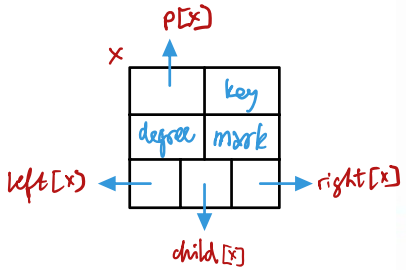
\includegraphics[width=0.5\linewidth]{Images/heap_di_fibonacci/nodo_heap.png}
 \end{figure}
Come possiamo vedere, questi nodi hanno vari campi:
\begin{itemize}
    \item \textbf{p[x]}: sostanzialmente è un puntatore al nodo padre.
    \item \textbf{left[x]|right[x]}: sono dei puntatori ai fratelli sinistri e destri. Naturalmente, scorrere la lista da sinistra o da destra non cambierà i nodi che troveremo dato che si tratta di una \textbf{lista circolare}.
    \item \textbf{child[x]}: puntatore che si riferisce al figlio di x. In questo caso ne abbiamo solo uno non perché i nodi possano avere un solo figlio, ma perché da questo troviamo tutti gli altri grazie ai campi left e right.
    \item \textbf{degree[x]|deg[x]}: sono entrambi lo stesso campo e vanno a dire il numero di figli che questi nodi hanno.
    \item \textbf{mark[x]}: questo è un campo booleano che ci dice se un nodo ha perso dei figli dall'ultima volta che è diventato a sua volta figli. Vedremo che grazie a questo campo potremo effettuare alcune procedure interessanti.
\end{itemize}

Definiremo, inoltre, la radice dello heap come $H.min$ o come $min[H]$ che conterrà, per l'appunto il minimo. Questo sarà l'unico accesso allo heap che avremo. E definiremo anche $H.n$ o $n[H]$ che indicherà il numero di chiavi in H. 
\begin{figure}[H]
    \centering
    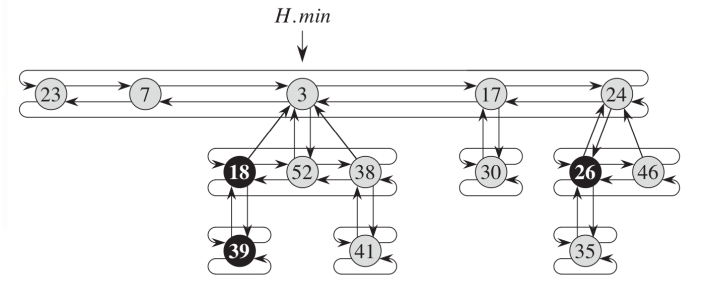
\includegraphics[width=0.5\linewidth]{Images/heap_di_fibonacci/lista_heap_esempio.png}
\end{figure}

\section{Funzione potenziale}
La funzione potenziale $\Phi$ che utilizzeremo sarà
\begin{align*}
    &\Phi(H)=t(H)+2m(H)\geq0 \\
    &t(H)=\text{\#alberi nella lista delle radici}\\
    &m(H)=\text{\#nodi marcati in H}
\end{align*}

Anche in questo caso, sappiamo per certo che se $\Phi(H_0)$ è l'heap di Fibonacci vuoto, allora avremo che $\Phi(H)\geq\Phi(H_0)\geq 0$. Per le analisi che effettueremo utilizzeremo un upper boud $D(n)$ sul massimo grado di un qualunque nodo nello heap di fibonacci con n nodi e, dimostreremo, che questo $D(n)=O(log(n))$.
\section{Alberi binomiali non ordinati}
Per ogni albero $k \in N$, esiste un albero \textbf{non ordinato} $U_k$ di grado k, definito come:
\begin{itemize}
    \item $U_0$ è un albero formato da un solo nodo.
    \item Dato $U_{k-1}$, definiamo $U_k$ come l'albero formato due copie di $U_{k-1}$ nel seguente modo
    \begin{figure}[H]
        \centering
       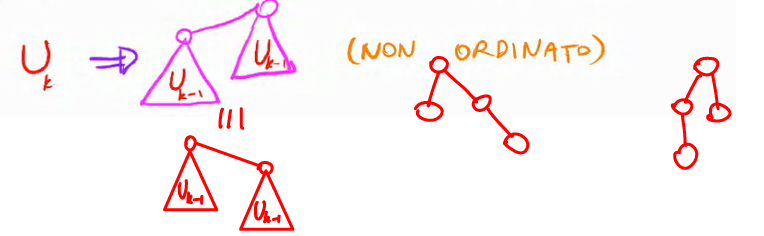
\includegraphics[width=0.5\linewidth]{Images/heap_di_fibonacci/creazione_u_k.png}
    \end{figure}

\end{itemize}
Anche in questo caso possiamo notare la presenza di alcune proprietà fondamentali che caratterizzano questi tipi di alberi. Per cui, per ogni $k=0,1,\ddots$ valgono:
\begin{itemize}
    \item $U_k$ ha $2^k$ nodi.
    \item L'altezza di $U_k$ è k.
    \item $U_k$ ha $\binom{k}{i}$ nodi a profondità $i$.
    \item La radice di $U_k$ ha grado k ed ogni altro nodo in $U_k$ ha grado inferiore a k. Inoltre i figli di $U_k$ sono radici di $U_0,U_1,\ddots,U_{k-1}$ ma \textbf{senza alcun particolare ordine}.
\end{itemize}

\section{Operazioni su Heap di Fibonacci}
Le principali operazioni che troviamo su questo tipo di strutture dati sono:
\begin{itemize}
    \item Make-Heap;
    \item Insert;
    \item Minimum;
    \item Extract-Min;
    \item Union;
    \item Decrease\_key;
    \item Delete.
\end{itemize}

Andando a considerare tutte le operazioni meno che decrease\_key e delete, avremo che lo heap di Fibonacci è una collezzione di alberi binomiali non ordinati. E, si osserva, che $D(n) = O(log(n))$ almeno quando lo heap è formato da alberi binomiali non ordinati e varrà che se $D'(n)$ è il massimo gradi di un nodo in uno heap senza mai usare operazioni di delete e decrease key, allora \[D'(n)\leq D(n)\].
Cominciamo ad analizzare le operazioni, partiamo con l'idea di ritardare il più possibile il lavoro di ristrutturazione dello Heap, per cui, molte operazioni che descriveremo adesso sembreranno particolarmente semplici dato che, il lavoro effettivo, verrà poi sviluppato in seguito.
\subsection{Make-Fibonacci-Heap()}
Questa operazione permette la creazione di un nuovo heap di Fibonacci inizialmente vuoto. 

\begin{algorithm}[H]
\caption{MAKE-FIBONACCI-HEAP()}
\begin{algorithmic}[1]
    \State $H \gets \textsc{Allocate-Node}()$
    \State $n[H] \gets 0$
    \State $min[H] \gets \textbf{NIL}$
    \State \Return $H$
\end{algorithmic}
\end{algorithm}
La complessità di questo algoritmo è banale, poiché $\Delta t = 0,\Delta m =0$ allora avremo che $\Delta\Phi=0$. Pertanto, $c'=c+\Delta\Phi=c=O(1)$.

\subsection{Fib-Heap-Insert($H,x$)}
Questa operazione inserisce un nuovo nodo all'interno dello heap inserendolo, semplicemente, all'iterno della lista iniziale e, se necessario, cambiando anche il minimo. 
\begin{algorithm}[H]
\caption{FIB-HEAP-INSERT($H, x$)}
\begin{algorithmic}[1]
    \State $degree[x] \gets 0$  \Comment{Settiamo tutti i parametri a 0 o NIL }
    \State $p[x] \gets \textbf{NIL}$
    \State $child[x] \gets \textbf{NIL}$
    \State $left[x] \gets x$
    \State $right[x] \gets x$
    \State $mark[x] \gets \textbf{false}$
    \State \textit{concatenate the root list containing $x$ with root list $H$}
    \If{$min[H] = \textbf{NIL}$ \textbf{or} $key[x] < key[min[H]]$} \Comment{Aggiorniamo il minimo}
        \State $min[H] \gets x$
    \EndIf
    \State $n[H] \gets n[H] + 1$ \Comment{Aggiorniamo il numero di nodi presenti}
\end{algorithmic}
\end{algorithm}
Analizzando la complessità, noteremo che questa volta $\Delta t = 1$ e non cambierà, però, $\Delta m$, dunque $\Delta \Phi = 1$. La complessità sarà, dunque, $c'=c+\Delta\Phi=c+1=O(1)$.
\subsection{Minimum(H)}
L'estrazione del minimo rimane banale poiché questa rimane sempre la radice del nostro Heap.
\begin{algorithm}[H]
\caption{FIB-HEAP-INSERT($H, x$)}
\begin{algorithmic}[1]
    \State return(min(H))
\end{algorithmic}
\end{algorithm}
La complessità sarà $\Theta(1)$ poiché la funzione potenziale rimane invariata.
\subsection{Fib-Heap-Union($H_1,H_2$)}
Questa è la procedura per cui due Heap di Fibonacci vengono uniti. Semplicemente, verrà creato un nuovo Heap e su questo si concateneranno le due liste scegliendo il giusto minore da utilizzare. 
\begin{algorithm}[H]
\caption{FIB-HEAP-UNION($H_1, H_2$)}
\begin{algorithmic}[1]
    \State $H \gets \textsc{Make-Fib-Heap}()$
    \State $H.min \gets H_1.min$
    \State \textit{concatena la lista delle radici di $H_2$ con la lista delle radici di $H$}
    \If{($H_1.min = \textbf{NIL}$) \textbf{or} ($H_2.min \neq \textbf{NIL}$ \textbf{and} $H_2.min.key < H_1.min.key$)}
        \State $H.min \gets H_2.min$
    \EndIf
    \State $H.n \gets H_1.n + H_2.n$
    \State \Return $H$
\end{algorithmic}
\end{algorithm}
La complessità in questo caso rimane $O(1)$ poiché non cambia il numero di alberi alla radice, considerando che $t(H) = t(H_1)+t(H_2)$ non stiamo aggiungendo alcun nodo rispetto a quelli già esistenti.
\subsection{Fib-Heap-Extract-Min(H)}
In questo momento arriva il lavoro più importante da considerare. Il problema nasce in questo momento dal fatto che, dopo aver estratto il minimo, noi non abbiamo idea di dove sia il nuovo valore minimo, per cui, abbiamo bisogno di effettuare una ricerca e, nel mentre, sistemare il tutto.
\begin{algorithm}[H]
\caption{FIB-HEAP-EXTRACT-MIN($H$)}
\begin{algorithmic}[1]
    \State $z \gets H.min$
    \If{$z \neq \textbf{NIL}$}
        \For{\textit{ciascun figlio $x$ di $z$}}
            \State \textit{aggiungi $x$ alla lista delle radici di $H$} \Comment{Tutti i figli vanno alla lista della radice}
            \State $x.p \gets \textbf{NIL}$
        \EndFor
        \State \textit{rimuovi $z$ dalla lista delle radici di $H$}
        \If{$z == z.right$} \Comment{Verifichiamo che non fosse l'unico elemento nella lista}
            \State $H.min \gets \textbf{NIL}$
        \Else
            \State $H.min \gets z.right$
        \EndIf
        \State \textsc{Consolidate}($H$) \Comment{Operazione di sistemazione dell'albero}
        \State $H.n \gets H.n - 1$
    \EndIf
    \State \Return $z$
\end{algorithmic}
\end{algorithm}

Vediamo quindi adesso la componente fondamentale della procedura che è il consolidamento della lista delle radici in cui si ripeteno i seguenti passi affinché ogni radice nella lista delle radici non avrà un \textbf{grado distinto}:
\begin{enumerate}
    \item  Trovare due radici x e y nella list adelle radici con lo stesso grado. E, supponiamo che $x.key \leq y.key$ senza perdere generalità.
    \item Colleghiamo y a x: eliminiamo y dalla lista delle radici e trasformiamo y in un figlio di x. Questa operazione è svolta dalla procedura di Fib-Heap-Link. L'attributi $x.degreee$ verrà incrementato e la marcatura di y sarà eliminata se presente.
\end{enumerate}

\begin{algorithm}[H]
\caption{CONSOLIDATE($H$)}
\begin{algorithmic}[1]
    \State \textit{Sia $A[0..D(H.n)]$ un nuovo array} \Comment{Array dei gradi}
    \For{$i \gets 0$ \textbf{to} $D(H.n)$} 
        \State $A[i] \gets \textbf{NIL}$
    \EndFor
    \For{\textit{ciascun nodo $w$ nella lista delle radici di $H$}} \Comment{Controlliamo per ogni nodo il suo grado nell'array}
        \State $x \gets w$
        \State $d \gets x.degree$
        \While{$A[d] \neq \textbf{NIL}$} \Comment{Se c'è un altro nodo con lo stesso grado di x}
            \State $y \gets A[d]$
            \If{$x.key > y.key$}
                \State \textit{scambia $x$ con $y$}
            \EndIf
            \State \textsc{Fib-Heap-Link}($H, y, x$) \Comment{Effettuiamo il Link}
            \State $A[d] \gets \textbf{NIL}$ \Comment{Resettiamo il grado nell'array}
            \State $d \gets d + 1$ 
        \EndWhile
        \State $A[d] \gets x$ \Comment{Aggiungiamo il nuovo grado nell'array dei gradi}
    \EndFor
    \State $H.min \gets \textbf{NIL}$  \Comment{Resettiamo il minimo}
    \For{$i \gets 0$ \textbf{to} $D(H.n)$} \Comment{Troviamo il nuovo minimo tra le radici}
        \If{$A[i] \neq \textbf{NIL}$}
            \If{$H.min == \textbf{NIL}$} \Comment{Primo nodo a venir visto}
                \State \textit{crea una lista di radici per $H$ che contiene solo $A[i]$}
                \State $H.min \gets A[i]$ 
            \Else
                \State \textit{inserisce $A[i]$ nella lista delle radici di $H$} \Comment{Via via, li andiamo inserendo nella lista}
                \If{$A[i].key < H.min.key$}
                    \State $H.min \gets A[i]$
                \EndIf
            \EndIf
        \EndIf
    \EndFor
\end{algorithmic}
\end{algorithm}

Per completezza, riportiamo anche la procedura di link.
\begin{algorithm}[H]
\caption{FIB-HEAP-LINK($H, y, x$)}
\begin{algorithmic}[1]
    \State \textit{Rimuove $y$ dalla lista delle radici di $H$}
    \State \textit{Trasforma $y$ in un figlio di $x$, incrementando $x.degree$}
    \State $y.mark \gets \textbf{false}$
\end{algorithmic}
\end{algorithm}

Andiamo ad analizzare la complessità di questa operazione. Per quanto riguarda l'extract min, vediamo che l'unica operazione rilevante è quella dove si spostano i figli della vecchia radice alla lista della radice e questa operazione ha complessità $O(D(n))$. 
Dopodiché, analizzando la consolidate troviamo:
\begin{itemize}
    \item $O(D(n))$ derivante dall'operazione di creazione dell'array dei gradi e la sua inizializzazione.
    \item $O(t(H))$ derivante dall'operazione di consolidamento effettivo dell'albero tramite i vari link.
    \item $O(D(n))$ derivante dalla ricerca del minimo nelle radici inserite che saranno $t(H)$.
\end{itemize}
Il costo reale sarà quindi
\begin{align*}
    &=O(D(n)) + \text{Derivante dall'operazione di estrazione del minimo}\\
    &+ D(n) + t(H) \text{Derivante dal processo di consolidamento delle radici}\\
    &= O(D(n)+t(H))
\end{align*}
Per un totale di:
\begin{align*}
    &\Delta t \leq (D(n)+1)-t(H) \quad \Delta m \leq 0\\
    &\Delta \Phi = \Delta t + 2 \Delta m \leq D(n)+1-t(H)\\
    &c' = c+\Delta \Phi = O(D(n)+t(H))+D(n)+1-t(H) = O(D(n))
\end{align*}
\subsection{Decrease Key}
L'operazione di Decrease key va a selezionare un nodo per poi diminuire la chiave. Una volta che questa è diminuita si controlla se è una radice e, se non lo è, allora si stacca il nodo mediante l'operazione di cut e poi si eseguono dei tagli a cascata. Infine, si controlla se il minimo è cambiato o meno.
\begin{algorithm}[H]
\caption{FIB-HEAP-DECREASE-KEY($H, x, k$)}
\begin{algorithmic}[1]
    \If{$k > x.key$}
        \State \textbf{error} "la nuova chiave è maggiore di quella corrente"
    \EndIf
    \State $x.key \gets k$
    \State $y \gets x.p$
    \If{$y \neq \textbf{NIL}$ \textbf{and} $x.key < y.key$}
        \State \textsc{Cut}($H, x, y$) \Comment{Inseriamo il nodo nella lista delle radici}
        \State \textsc{Cascading-Cut}($H, y$) 
    \EndIf
    \If{$x.key < H.min.key$}
        \State $H.min \gets x$ \Comment{Se è cambiato il minimo, lo aggiorniamo}
    \EndIf
\end{algorithmic}
\end{algorithm}
\begin{algorithm}[H]
\caption{CUT($H, x, y$)}
\begin{algorithmic}[1]
    \State \textit{Rimuove $x$ dalla lista dei figli di $y$, decrementando $y.degree$}
    \State \textit{Aggiunge $x$ alla lista delle radici di $H$}
    \State $x.p \gets \textbf{NIL}$
    \State $x.mark \gets \textbf{false}$
\end{algorithmic}
\end{algorithm}
\begin{algorithm}[H]
\caption{CASCADING-CUT($H, y$)}
\begin{algorithmic}[1]
    \State $z \gets y.p$
    \If{$z \neq \textbf{NIL}$}
        \If{$y.mark == \textbf{false}$}
            \State $y.mark \gets \textbf{true}$
        \Else
            \State \textsc{Cut}($H, y, z$)
            \State \textsc{Cascading-Cut}($H, z$)
        \EndIf
    \EndIf
\end{algorithmic}
\end{algorithm}
Analizziamo la complessità di questa procedura. Finalmente entra in gioco la questione dei nodi marchiati per cui vedremo che cambierà la complessità. Supponiamo che CUT abbia costo costante e dia vita a d cascading cut. Consideriamo che al più un nodo verrà marcato ma almeno $d-1$ verranno smarcati dai tagli a cascata per cui:\[\Delta m \leq 1 - (d-1)=2-d\] 

Supponiamo quindi che la procedura cascading cut venga richiamata d volte. Avremo che il costo reale sarà $\Theta(d)$, per cui:
\begin{align*}
    &\Phi(H) = t(H)+2m(H)\\
    &\Phi(H') \leq (t(H)+d)+2(m(H)-(d-1)+1)=\\
    &= t(H)+d+2m(H)-2d+2+2=\\
    &= t(H)+2m(H)-d+4
\end{align*}
Per cui, segue che $c' = O(d)+\Phi(H')-\Phi(H)=O(d)-d+4=O(1)$
\subsection{Delete}
Infine, banalmente avremo la delete che consiste semplicemente in una decrease key al minimo possibile per poi effettuare un'estrazione del minimo.
\begin{algorithm}[H]
\caption{FIB-HEAP-DELETE($H, x$)}
\begin{algorithmic}[1]
    \State \textsc{Fib-Heap-Decrease-Key}($H, x, -\infty$)
    \State \textsc{Fib-Heap-Extract-Min}($H$)
\end{algorithmic}
\end{algorithm}

La complessità di questa operazione sarà $O(D(n))$.

\section{Proprietà di Fibonacci}
Definiamo la serie di Fibonacci in questo modo:
\begin{align*}
    &F_0 = 0,\quad F_1 = 1\\
    &F_k = F_{k-1}+F_{k-2} \quad k\geq 2\\
\end{align*}

\textbf{Lemma 1}\\
Questo primo lemma ci dice che $F_{k+2} = 1+ \sum_{0}^{k}F_i \quad k\geq0$.\\
\textbf{Dimostrazione}\\
Caso base: k = 0
\[F_{k+2}=F_2=0+1=1 \xrightarrow{} 1+\sum_{0}^{k}F_i = 1+ \sum_{0}^{0}F_i=1+0=1\]
Passo induttivo: \\
\[F_{k+1+2}=F_{k+3}=F_{k+2}+F_{k+1}=1+\sum_{0}^{k}F_i+F_{k+1}=1+\sum_{0}^{k+1}F_i\]

Prima di procedere con il prossimo lemma, andiamo a fare alcune considerazioni su quello che viene definto il \textbf{rapporto aureo}. Infatti, questo è strettamente legato alla serie di Fibonacci come vedermo.
Il valore del rapporto aureo è $\Phi=\frac{1+\sqrt{5}}{2}$ e, si può dimostrare che $1+\Phi=\Phi^2$. Inoltre, è importante affermare che $2>\Phi$.\\
\textbf{Lemma 2}\\
$F_{k+2} \geq \Phi^k$ per $k\geq0$
\\
\textbf{Dimostrazione}\\
Caso base: k = 0
\begin{align*}
    &k=0:\quad F_{k+2} = F_2 = 1 = \Phi^0 = \Phi^k\\
    &k=1:\quad F_{k+2} = F_3 = 2 > \Phi = \Phi^1 = \Phi^k
\end{align*}
Passo induttivo: $k\geq1$ e, ipotesi induttiva: $F_{h+2}\geq \Phi^h \forall 0\geq h < k$.
\begin{align*}
    &F_{(k+1)+2} = F_{k+3} = F_{k+1}+F_{k+2}=\\
    &=F_{(k-1)+2}+F_{k+2}\geq \Phi^{k-1} + \Phi^{k}=\\
    &=\Phi^{k-1}(1+\Phi)= \Phi^{k-1}\Phi^2 = \Phi^{k+1}
\end{align*}
\textbf{Lemma 3}\\
Sia x un nodo in uno heap di Fibonacci e sia $degree[x] = k$, siano $y_1,\dots y_k$ i figli di x nell'ordine in cui sono stati innestati in x. Allora $degree[y_i]\geq i-2$, per $i=3,4,\dots k$.\\
\textbf{Dimostrazione}\\
Sia $i\geq3$, notiamo che quando $y_i$ è innestato in x al tempo T, il nodo x ha già $y_1,\dots, y_{i-1}$ tra i suoi figli, per cui $degree_{t-1}[y_i]=degree_{t-1}[x] \geq i-1$. Dall'istante T, $y_i$ può aver perduto al più un figlio e, quindi, $degree[y_i]\geq i-2$.
\begin{figure}[H]
    \centering
    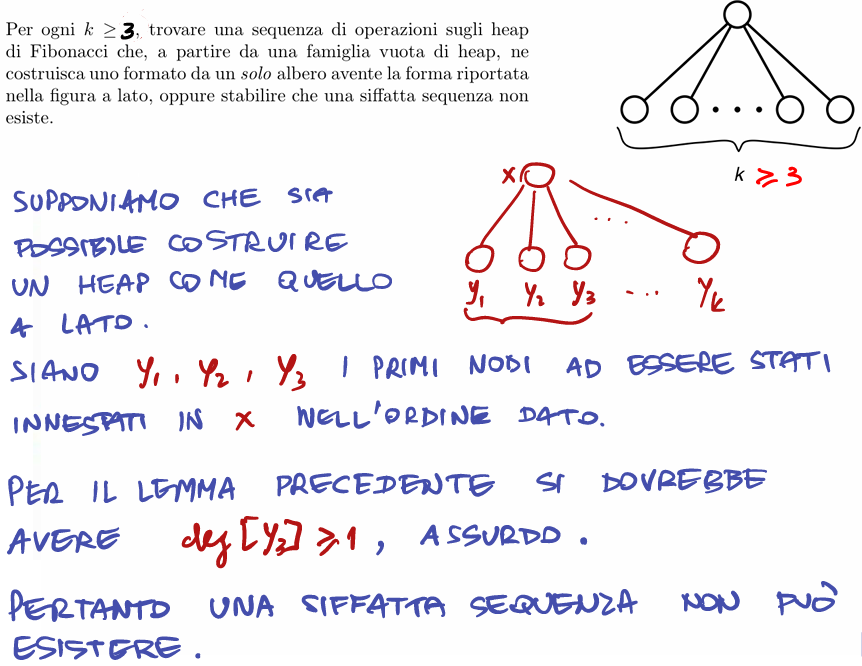
\includegraphics[width=0.8\linewidth]{Images/heap_di_fibonacci/esercizio_fibonacci_terzo.png}
\end{figure}
\textbf{Lemma 4}\\
Sia x un nodo in uno heap di Fibonacci e sia $degree[x] = k$, allora $size[x] \geq F_{k+2}$, dove $size[x]$ è il numero di nodi nel sottoalbero radicato in $x$.
\textbf{Dimostrazione}\\
Innanzitutto poniamo:
\begin{align*}
    &s_j=min.size[z]\\
    &degree[z] = j\\
    &z \in H\\
    &H \in H_u \quad H_u = \text{Famiglia di tutti gli Heap di Fibonacci}
\end{align*}
Si ha che 
\[s_0=1, s_1 \geq 2, \quad s_{j+1}\geq s_j \quad j \in N\] 
L'obiettivo sarà quindi dimostrare che 
\[s_k \geq F_{k+2} \quad \text{ se } deg[x] = k, \quad size[x]\geq s_k \geq F_{k+2}\]

\textbf{Dimostrazione}\\
Dimostriamo innanzitutto che \[s_0=1, s_1 \geq 2, \quad s_{j+1}\geq s_j \quad j \in N\]

Se $k=0$, allora vuol dire che $degree[x] = 0$, per cui, il nodo non ha alcun figlio e, quindi $size[x] = 1$.\\
Se $k=1$, allora $degree[x] = 1$, quindi x ha un solo figlio, per cui $size[x] \geq 2 $
\\
Andiamo adesso per induzione, per cui, suppinamo l'ipotesi $size[x] \geq F_{j+2}$, sia corretta per ogni $j<k$.
\begin{figure*}
    \centering
    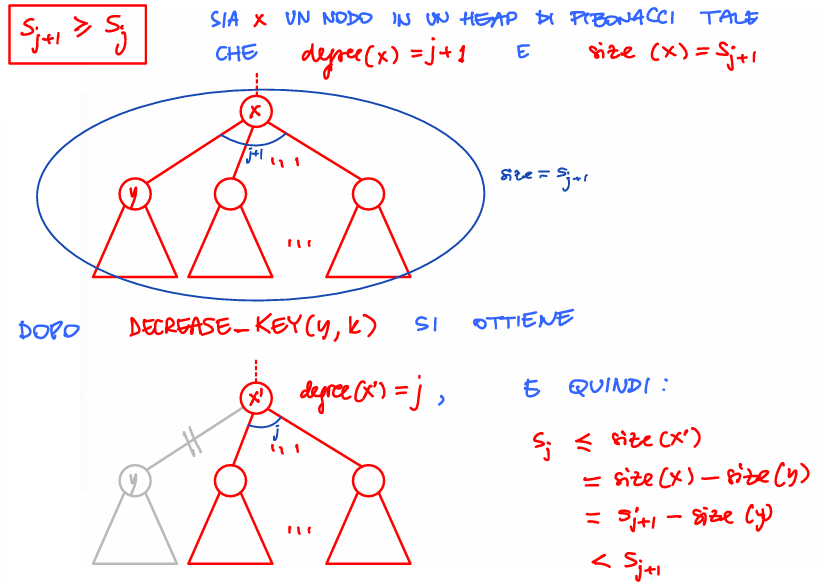
\includegraphics[width=0.8\linewidth]{Images/heap_di_fibonacci/s_j+1_maggiore_sj.png}
\end{figure*}
Dimostriamo che $s_j \geq F_{j+2} \quad \forall j=0,,1\dots$.
\begin{align*}
    &j=0 : \quad s_j = 1, \quad F_{j+2} = 1\\
    &j=1 : \quad s_j \geq 2, \quad F_{j+2} = F_3 = 2\\
    &j\geq 2 : s_j = size[y_1]+size[y_2],+\dots+size[y_j] + 1 \geq \quad \text{Segue dal lemma 3}\\
    &\geq 1+ s_{2-2}+s_{3-2}+\dots+s_{j-2}+1 =  \quad \text{Siccome $s_j\geq F_j+2$, possiamo applicare il Lemma 1}\\
    &= 2 + \sum_{i=2}^j s_{i-2} \geq 2+ \sum_{i=2}^j F_i = 1+ \sum_{i=0}^j F_i = F_{j+2}
\end{align*}
Poiché $degree[x] = k$ si ha che $size[x] \geq s_k \geq F_k+2$.
\\
\textbf{Corollario 1}\\
$size[x] \geq \Phi^{degree[x]}$\\
\textbf{Corollario 2}\\
$D(n)\leq \lfloor log_\Phi(n) \rfloor$ da cui $D(n) = O(log(n))$.\\
\textbf{Dimostrazione}\\
Sia x un nodo in uno heap di Fibonacci con n nodi. Si ha che $n \geq size[x]\geq \Phi^{degree[x]}$, pertanto:
\begin{align*}
    &degree[x] \leq \lfloor log_\Phi(n) \rfloor\\
    &D(n) = \max degree[x] \leq \lfloor log_\Phi(n) \rfloor
\end{align*}